\chapter{Numeric Evaluation of the Model for General Barriers}
\label{numeric_model}
This section will introduce two numeric approaches to the problem of reaction rates over fluctuating boundaries as outlined in the introduction \ref{mini_model}. The first method builds on the integration of the stochastic differential equation for a composite Markov process, the second method uses the macroscopic description of the same process in terms of partial differential equations \eqref{fpmeq1}. Both methods aim to approach the following model.\\

\begin{minipage}[t]{.5 \textwidth}
    \begin{figure}[H]
 \hspace{-1.8 cm}       \input{plots/abSkizze.pdf_tex}
    \end{figure}
\end{minipage}\hspace{0.05 \textwidth}\begin{minipage}[t]{.45\textwidth}
    \begin{figure}[H]
        \caption{Illustrative sketch of the system. The spherical sink of radius $R_s$ is surrounded by a (not necessarily) step shaped potential barrier with boundaries at $r=a$ and $r=b$. The potential fluctuates between different heights subject to a transition rate matrix with entries $\mathbb{W}_{mm'}$ (to keep things clear only two states are depicted here). This setup is embedded in a bath of Brownian particles with fixed density at $r \rightarrow \infty$. The particles move under the influence of the potential in its current state. The reaction rate $K$ is given by the number of particles per unit time that cross the barrier and hit the sink.\label{skizze}}
    \end{figure}
\end{minipage}

\section{Model Description}
\label{Model_Description}
The system under consideration consists of a spherical sink of radius $R_s$ that is surrounded by a potential barrier. The barrier is assumed to be of boxcar shape with limiting radius $a,b>R_s$ as illustrated in figure \ref{skizze}. It fluctuates between $M$ states with different height $U_m \in [U_0, \cdots U_M]$. The transition rates between potential states are given by a transition rate matrix $\mathbb{W}$ which is assumed to satisfy the detailed balance property \eqref{detailed_balance}. This system is embedded in a reservoir of Brownian particles. \\
It is desired to find the steady state rate $K$ at which the particles cross the barrier and hit the sink.\\
Therefore the state of the system is described as a composite Markov process as outlined in section \ref{Multivariate_Markov_Processes} in one spacial variable $\vec{r}$ and one discrete variable $m$ for the state of the barrier.
The appropriate boundary conditions in this case are for the probability density function (PDF) of the Brownian particles to vanishes at the sink boundary and to take a constant finite value for $|\vec{r}| \rightarrow \infty$. \\
\section{Brownian Dynamics}
\label{BDsim}
The term \textit{Brownian Dynamics Simulation} refers to the integration of the overdamped Langewin equation \eqref{BD1} i.e. the motion of particles with respect to a Gaussian random force. Therefore the equation for the diffusive coordinate $r_n$ of the Brownian particles is discretized in time, such that the actual discrete equation of Motion has the Form
\begin{equation}
    \vec r_m(t + \Delta t) = \vec r_m(t) - \frac{\vec \nabla U_m(\vec r)}{\gamma}\Delta t + \sqrt{2 D \Delta t} R(t)
    \label{discrete_eqm}
\end{equation}
where $R(t)$ is a Gaussian random process with zero average and $\sigma = 1$. $m$ denotes the reactive coordinate of the Brownian particle. This coordinate is updated in each time step with respect to the appropriate Master equation. This is done via a probabilistic scheme. For each time step and each particle one draws a random number $X$ from an uniform distribution on the interval $[0,1]$. Then one splits the interval $[0,1]$ into $M$ subintervals with size relative to the transition rates $\mathbb{W}_{i,j}$ depending on the state $j$ of the appropriate particle:
\begin{equation}
    \frac{1}{\sum_{m}^{M}\mathbb{W}_{m,j}} [\mathbb{W}_{1,j}, \mathbb{W}_{2,j}, \cdots , \mathbb{W}_{M,j}]
    \label{num_meq}
\end{equation}
and checks in which of the intervals the random number $X$ lies. The state of the particle is then updated to $i$.\\
This is probably the most trivial numerical solution to the given problem, but since the substrate particles do not interact it is still sufficient to evaluate the situation.

\subsection{Boundary Conditions}
Since we are looking for a steady state solution we must make sure that the number of particles is conserved. Therefore the flux of particles out of the simulation domain through the surface of the sink must equal the flux of particles into the simulation domain through its outer boundary.
Also, it proves appropriate to use spherical simulation domain of Radius $R_d$ with the sink of radius $R_s$ in its center to preserve the spherical symmetry of the anticipated solution.
Keeping these necessities in mind the boundary conditions at the sink surface and at the outer domain boundary are implemented as follows: \\
\begin{itemize}
    \item particles are reflected at the outer simulation boundary:
        \begin{lstlisting}
        r = SQRT(DOT_PRODUCT(par(:),par(:)))
        IF(r>Rd) THEN
            rnew = 2*Rd - r
        ENDIF
        \end{lstlisting}
        where par(:) are the particles x,y and z coordinate, r is therefore the particles radial position after an integration step of the integration of the eqm.
    \item If the trajectory that connects the position of a particles before (A) and after (B) an integration step crosses the boundary of the sink the particle is reset to a distance $R_s - r$ of the outer boundary of the simulation domain:
        \begin{lstlisting}
        A   = parold(:)
        B   = parnew(:)
        AB  = parold(:) - parnew(:)

        px = A + DOT_PRODUCT(A,AB)*AB/DOT_PRODUCT(AB,AB)

        IF( DOT_PRODUCT( px-A),(px-B)) < 0 )THEN
            r = SQRT(DOT_PRODUCT(px,px))
        ELSEIF( DOT_PRODUCT( px-A),(px-B)) >= 0 )THEN
            r = SQRT(DOT_PRODUCT(B,B))
        ENDIF
        
        IF(r<Rs) THEN
            rnew = Rs + Rd - r
        ENDIF
        \end{lstlisting}
        This fragment of code calculates the closest point px to the sink center on the line containing A and B. Then it checks, if this point px is between A and B. Based on this, it updates the radial position of the particle to set it to the boundary of the simulation domain, if it crossed the boundary of the sink.
\end{itemize}
\subsection{Potential Barrier}
The potential $U_m(r)$ is set to be a modified Gaussian:
\begin{align}
    U_m(r) &= U_m \cdot \exp \left[-\left( \frac{r-\alpha}{\beta} \right)^{2n}\right], \nonumber \\
    \alpha &= a + \frac{b-a}{2}, \nonumber \\
    \beta  &= \frac{b-a}{2}.
    \label{mod_gauss}
\end{align}
This is a regular Gaussian bell for $n=1$ and converges to a step potential for $n\rightarrow \infty$. \\
Since for large $n$ the shape of the potential can not be resolved by the trajectories of the Brownian particles (unless the time step is set very small which is computationally inefficient) it is useful to implement the potential barrier via transition probabilities for the diffusing particles across the barrier boundaries. The reasoning that is commonly employed in this situation is that of local equilibrium \cite{glansdorf1971} that allows to implement the transition of particles over the jump discontinuities of the potential as follows: \\
If a particle in state $m$ crosses the boundary of the potential barrier from a lower to a higher level, it has a probability $P_r = P_{\Delta U_m}$ to be reflected and a probability $P_p = 1 - P_{\Delta U_m}$ to pass where $P_{\Delta U_m}$ is given by an Arrhenius factor
\begin{equation}
    P_{ \Delta U_m} = \exp \left[\frac{\Delta U_m}{K_B T}  \right].
    \label{arrhenius_factor}
\end{equation}
If a particle crosses the boundary of the potential barrier from a higher to a lower level it does so with probability $P_p = 1$.
Why this form of the boundary conditions holds in this particular case will be discussed in more detail in section \ref{Fit_Conditions}.
\subsection{Density Profile}
To calculate the radial density profile of the substrate particles one bins their radii at each time step and normalize the resulting histogram to its volume per bin. This is averaged over each time step after a certain equilibration time of the simulation.
\subsection{Adsorption Rate}
To calculate the adsorption rate, we simply count the number of particles that crosses the sink surface and is set to the simulation boundary. This number is then normalized to the time per time step and averaged over each time step after a certain equilibration time of the simulation.
\subsection{Error estimation}
To calculate errors for the correlated time series of measurements of $\rho(r)$ and $K$, Jackknife binning, block averages and correction for autocorrelation from the statistics package provided by Burkhard Bunk are used \cite{bunk2006}.
\section{Method of Lines}
\label{method_of_lines}
The method of lines \cite{pregla1989, saucez2001} is a technique for solving partial differential equations that are well posed as an initial value problem in at least one dimension. It uses spatial discretization of the derivatives in all but other dimensions and then treats the resulting semi discrete problem as a system of coupled ordinary differential equations. This has the advantage, that it is possible to use highly optimized methods that have been developed for numeric integration of ordinary differential equations for the treatment of partial differential equations.\\
Since the time dependent description of the system: 
\begin{align}
    \frac{\partial}{\partial t } \rho_n(r,t) =   &- \vec{ \nabla } \left[\frac{1}{\gamma}\vec{f}(\vec{x},n,t)\rho_n(r,t) \right] +\vec{\nabla}^{2}\left[ D\rho_n(r,t) \right] \nonumber \\
    &+ \sum_{n'} \left\{ W_{nn'}\rho_{n'}(r,t) - W_{n'n}\rho_n(r,t)\right\}.
    \label{fpmeqmol}
\end{align}
together with arbitrarily chosen initial conditions:
\begin{equation}
    \rho_n(r,t_0) = \rho_n^{(0)}(r)
    \label{rho0mol}
\end{equation}
and the boundary conditions \eqref{bcrs} and \eqref{bcinf} fulfills the requirement of being a initial value problem in one dimension (the time dimension in this case) it is possible to treat it using the method of lines to obtain a solution for the density profiles.\\
The resulting reaction rates can then be calculated using equation \eqref{Rate}.\\
Since the solution of this type of Fokker-Planck system is unique \cite{soize1994}, and is also a global attractor \cite{Efendiev2000}, the choice of the initial condition does only influence the time that the system needs to converge to the steady state.\\
For technical details of the implementation of the method please refer to the documentation of {\tt Mathematica} 9\textsuperscript{\textregistered}. The options used with {\tt NDsolve} to obtain the results presented in this thesis are the following:\par
{\tt    MaxSteps $\rightarrow$ Infinity,  \\
        MaxStepFraction $\rightarrow$ 0.002, \\
        AccuracyGoal $\rightarrow$ 15,  \\
        StartingStepSize $\rightarrow$ 0.001, \\
        WorkingPrecision $\rightarrow$ MachinePrecision, \\
        Method $\rightarrow$ \{``MethodOfLines'', \\
            ``SpatialDiscretization'' $\rightarrow$ \{``TensorProductGrid'', \\
            ``MinPoints'' $\rightarrow$ 10000\}\}}

\section{Comparison of Models}
The two computational models described in this chapter both target the same problem but with a fundamentally different approach. Brownian Dynamics simulations integrate the underlying stochastic differential equations whereas the Method of Lines solves the equivalent partial differential equations. Therefore the Brownian Dynamics approach allows for the calculation of microscopic quantities such as locally resolved mean square displacement of particles whilst the Method of Lines approach only gives access to macroscopic quantities such as fluxes and density profiles. The advantage of the Method of Lines lies in its efficiency. With Brownian dynamics Simulations the errors in all calculated quantities scale with $N^{-1/2}$ with $N$ being the number of simulated particles. If the particles do not interact, the time $T$ for the simulation scales linear with $N$ and therefore the precision of the results will also go with $T^{-1/2}$. Although the documentation of Mathematica does not tell much about the actual routines in use for the implementation of the Method of lines they are empirically observed to be a lot more efficient than BD Simulations when it comes to derive solutions up to a required precision of accuracy. Otherwise the results of the two procedures are in good agreement as illustrated by the results depicted in figure \ref{Rho_numeric}.\\
For this reason the method of lines will be used to calculate numeric results for macroscopic quantities and Brownian Dynamic simulations will only be used if it is necessary to explicitly calculate microscopic quantities.

\section{First Results}
The advantage of a numeric approach is that it offers a first impression of the behavior and the features of a given system without any further analytic work involved. Therefore a minimal setup consisting of a repulsive barrier that switched between two states $U_1 = 0$ and $U_2 = 3 K_B T$ with boundaries at $a = 6 R_s$ and $b = 11 R_s$ and exponent $n=32$ was treated by both the Brownian dynamics (BD) and the Method of lines (MOL) procedure for symmetric switching rates $W_{12} = W_{21} = W$. The results are given in figure \ref{Rho_numeric} for different values of the switching rate $W$. 
\begin{minipage}[t]{.66 \textwidth}
     \begin{figure}[H]
        \hspace{-1.2cm } 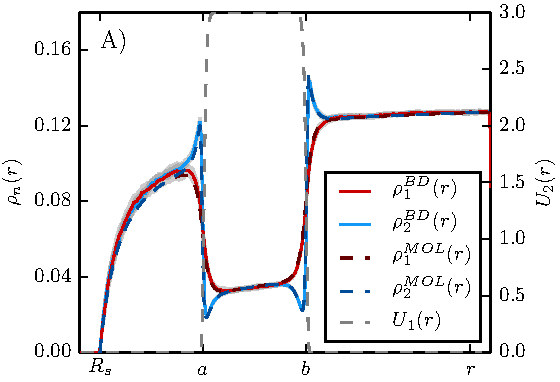
\includegraphics[width = 1 \textwidth]{plots/rd025_numeric.pdf} \\
        \vspace{.4 cm} \hspace{-1.2cm } 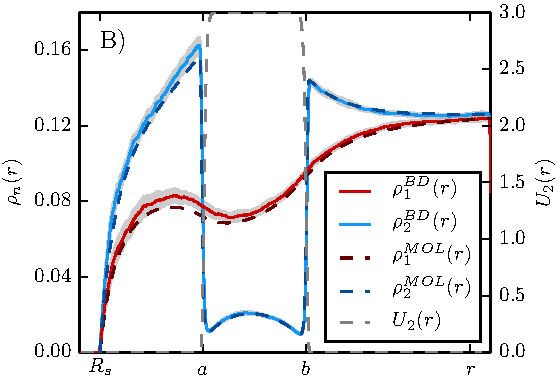
\includegraphics[width = 1 \textwidth]{plots/rd25_numeric.pdf} \\
        \vspace{.4 cm} \hspace{-1.2cm } 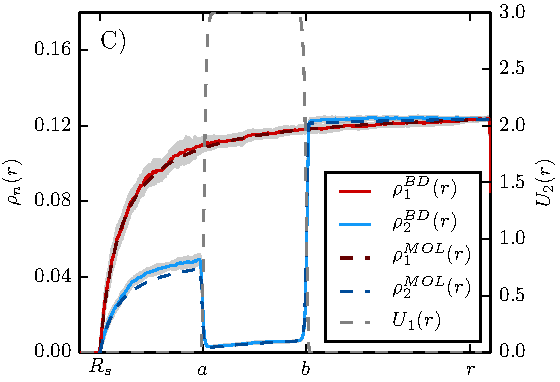
\includegraphics[width = 1 \textwidth]{plots/rd250_numeric.pdf}
    \end{figure}
\end{minipage}\hspace{-0.2 cm}\begin{minipage}[t]{.37 \textwidth}
    \begin{figure}[H]
        \caption{Comparison of density profiles obtained by Brownian dynamics simulations (BD) and by the numerical method of lines (MOL) for different values of the switching rate, A: $W=2 \times 10^{2}/\Delta t$, B: $W=2/\Delta t$, and C: $W=2 \times 10^{-3}/\Delta t$. The errors for BD are $2 \sigma$. The potential barrier has the shape of a generalized Gaussian \eqref{mod_gauss} with parameters $a = 6 R_s$, $b = 11 R_s$, $n = 32$ and two states of height $U_1 = 0$ and $U_2 = 3 K_B T$. The density profiles are given separately for particles in state 1 not interacting with the potential barrier ($\rho_1(r)$) and particles in state 2 $\rho_2(r)$ that have to overcome the barrier to reach the sink. Other parameters are $D = 0.025 R_s^2/\Delta t$, $\Delta t = 3 \times 10^{-3}$, $R_d = 30 R_a$ and $N = 1.5\times 10^{4}$ particles in case of the BD simulation. Initial conditions for BD are given by positioning all particles at the outer boundary of the simulation domain, initial conditions for the MOL  are given by a flat density distribution between the outer barrier boundary and the boundary of the simulation domain. The BD simulations were integrated from $t=0$ to $t=5 \times 10^3$ to equilibrate before measurement, the MOL runs were integrated up to $t = 10^{3}$ until convergence.\label{Rho_numeric}} 
    \end{figure}
\end{minipage}
\newpage
The resulting density profiles are given separately for particles in state 1 that diffuse freely and particles in state 2 that are inhibited by the repulsive barrier. Depending on the switching rate of particles between these states the density profiles very different qualitative signatures.
For fast switching rates  (figure \ref{Rho_numeric} A) the density profiles are very similar, only diverging at the boundaries of the potential barrier. For very slow switching rate (figure \ref{Rho_numeric} B) the density profiles are seemingly independent such that one of them resembles the solution for the ideal Smoluchowski problem as ilustrated in figure \ref{fig:rho_smoluchowski} and the other one resembles that of the Debye density profiles for a repulsive barrier as depicted in figure \ref{fig:rho_debye}. For intermediate switching rates (figure \ref{Rho_numeric} C) the density profiles exhibit more complex behavior not as tightly coupled as in the first case but still not completely independent as in the latter. It will become obvious in the latter that this behavior has a profound impact on the diffusion controlled reaction rate over the fluctuating barrier.


\section{Summary}
The previous chapter introduced two different numeric approaches to the problem of reaction rates over fluctuating barriers. First Brownian Dynamics sumulations building on the integration of integration of the underlying stochastic differential equation and thus describing the problem in the microscopic picture and second, the numerical Method of Lines for the integration of the partial differential equations for the time evolution of the density distribution of the system therefore describing it in a macroscopic picture. Results from both methods are shown to be in good agreement and exhibit interesting features in radial particle density distributions depending on the switching rate of the barrier.

